\begin{figure}[!]
\begin{center}
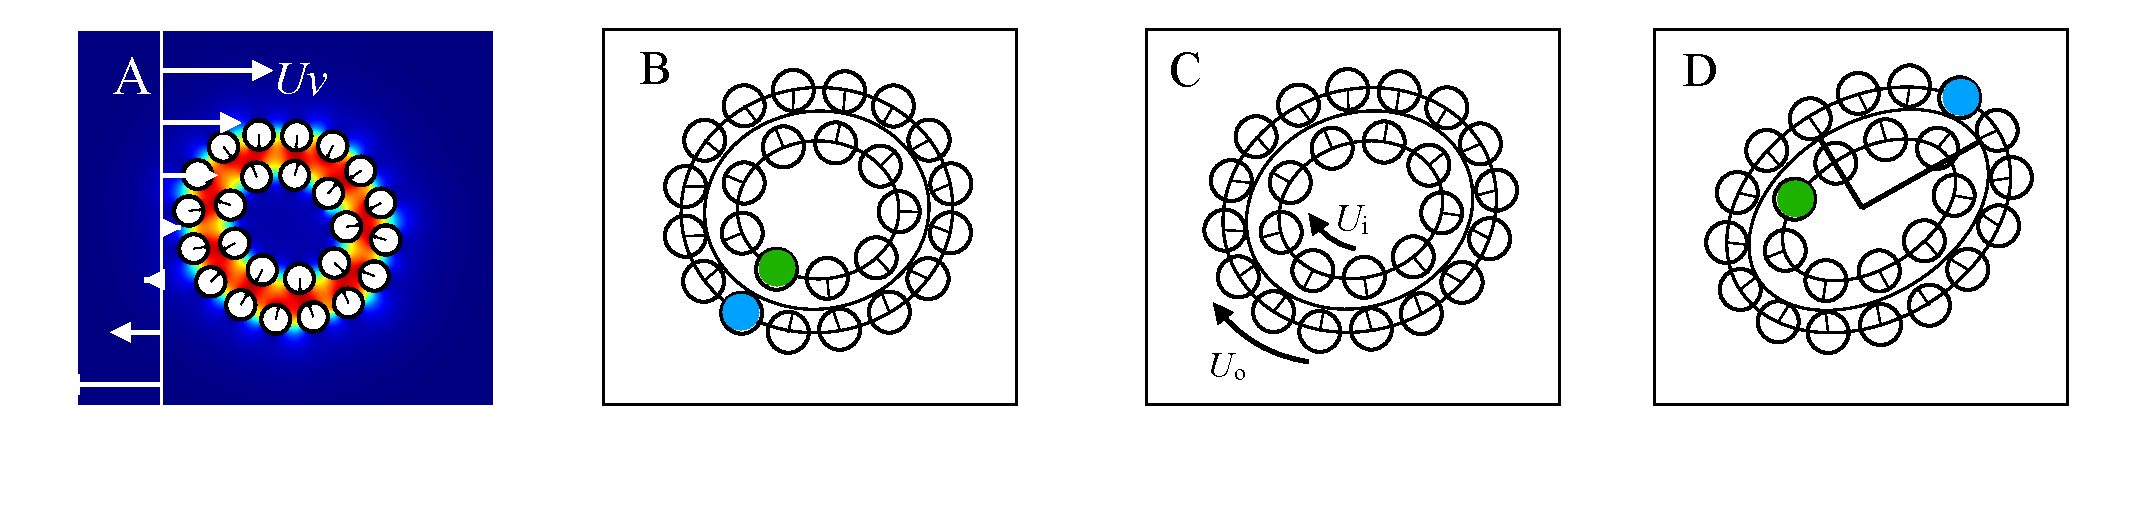
\includegraphics[width=1\textwidth]{figures/PW_fig1A-D.pdf}
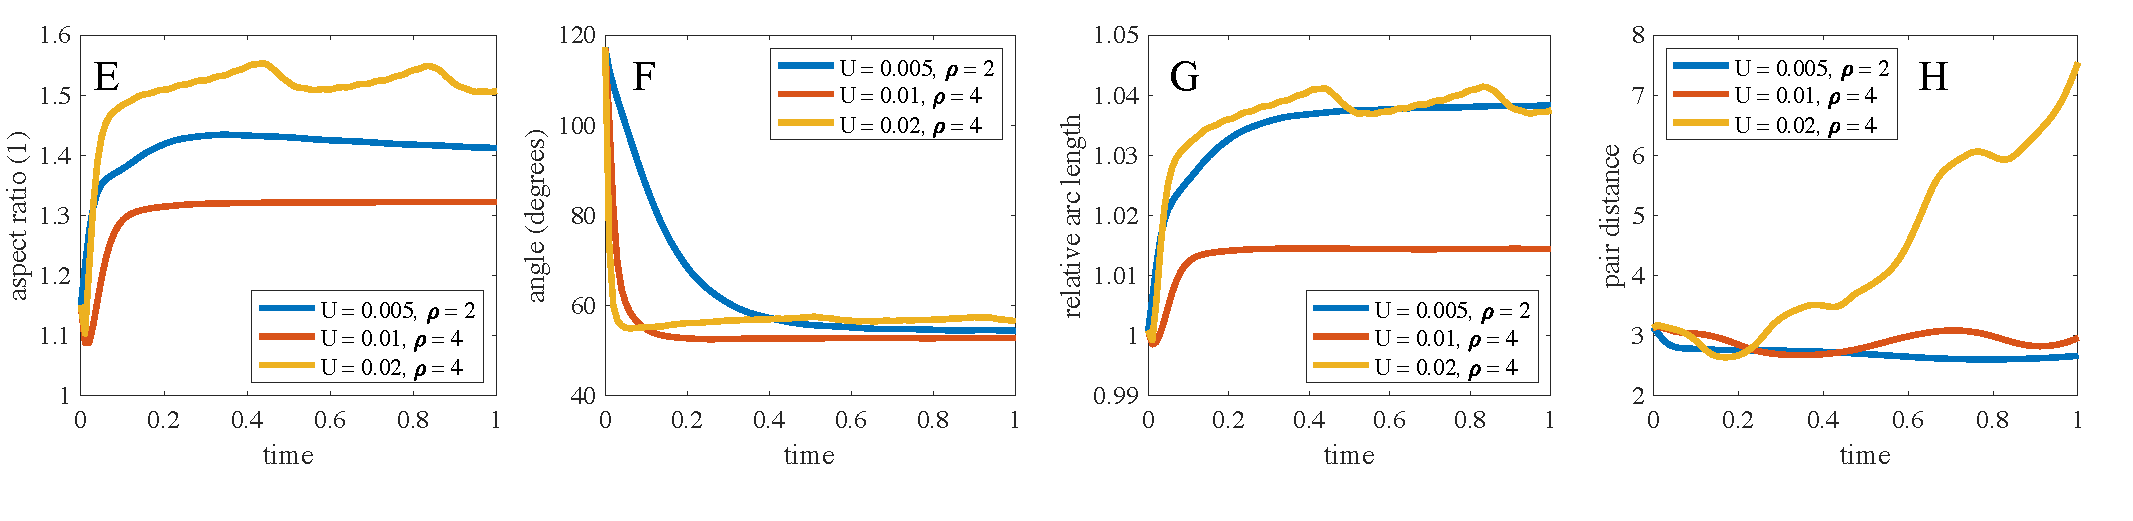
\includegraphics[width=1\textwidth]{figures/PW_fig1E-H.pdf}
\end{center}
\vspace{-0.3in}
\caption{\label{fig:tanktreading}\footnotesize (A) A vesicle formed by
  amphiphilic particles in shear flow, and the tank-treading motion
  (B)--(D). The separation of particle pairs in (B) and (C) illustrate
  inter-leaflet slip.  (E)--(G) Tank-treading reaches a steady state in
  elliptical aspect ratio, major-axis angle, and circumference.}
\end{figure}

\section{Preliminary work}
\subsection{Estimating two-dimensional elastic
moduli}
%\section{Preliminary Work on Two-dimensional Vesicle Hydrodynamics in Shear Flow\label{sec:preliminary_work}} 
%\section{Preliminary work on elastic moduli}
To derive a bending modulus, we first considered a planar bilayer subject to a uniform vertical load on the particle centers (Figure \ref{fig:bend}). 
Using a clamped condition at one end, the restoring force in the free part of the bilayer opposes the load.
For small deformations, it is possible to solve the bilayer loading in closed form, and 
this analytical solution (red curve) basically overlaps the midplane of the particle based solution (Figure \ref{fig:bend}A).
We thereby derived a bending modulus $\KB$ in the range 8.51--13.54 \kBT. Throughout the proposal, \kBT\; = 4.11$\times 10^{-21}$ J.
Experimental measurements have accurately determined the bending modulus for several lipid types, with 
typical values lying around 10 \kBT\; \cite{Naetal15,VeBrPa15,NAGLE2000159,PhysRevLett.113.248102}.

We also considered the stretching and tilt deformations \cite{Fu2018_SIAM}. 
Stretching occurs whenever there is an excess monolayer area,
and it is energetically costly since it exposes hydrocarbon tails to water.
To measure an area modulus, we stretched a circular vesicle, modeling the cross-section 
of a bilayer tube (Figure \ref{fig:bend}B \& C).
This procedure gave a monolayer area modulus 
34 $\pm$ 2 \kBT \;nm$^{-2}$. Manipulation experiments give a monolayer area modulus in the range 
30--40 \kBT\; nm$^{-2}$ \cite{Nagle17, Nagle17-2}. 

Finally, we considered the tilt deformation by applying a fixed tilt angle boundary condition. 
This boundary condition produces a tilt field that decays with the length scale $l = \sqrt{\KB/\KTH}$ 
Fitting to this field, our particle based simulation gave $\lambda = 1.2$ nm, which matches
the value $\KTH \approx 10$ \kBT \; nm$^{-2}$ reported in the literature \cite{KUZMIN2005, KoNa15}.

Our preliminary work is encouraging because in all cases, the bending, stretch, and tilt elastic moduli for the collection of amphiphiles
were in excellent agreement with the experimental values. This fact is especially remarkable 
since we assigned the main model parameters $\rho$ and $\gamma$ reasonable physical values, rather than using them as tuning parameter. 
Nevertheless, the characterization of material properties is incomplete. For one, the preliminary simulations involved relatively low particle numbers (20 to 30), and so we still need to
perform convergence studies with large particle-number systems to arrive at conclusive results. Secondly, we have yet to establish a functional
relationship between the model parameters and elastic moduli. Finally, to have relevance in physics and biology
we must incorporate the remaining twist and saddle splay deformations.
The following simulation outline shows how will achieve aims.

\subsection{Two-dimensional vesicle hydrodynamics in shear flow} 
%The motion of vesicles in shear flow is an important
%problem in the applied mathematics because simulations can reveal mechanical
%properties of membranes and lead to an enhanced understanding of 
%deformable particle laden flows \cite{Sinha15}. 
%
%
\begin{wrapfigure}[10]{r}{0.2\textwidth}
\centerline{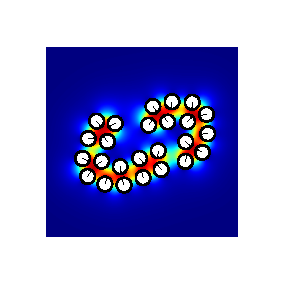
\includegraphics[width=0.2\textwidth]{figures/PW_fig5.pdf}}
\vspace{-8pt}
\caption{\label{fig:rupture} \footnotesize Rupture of tank-treading vesicle under strong shear flow.}
\end{wrapfigure}
%
To implement a vesicle in shear flow in the context of hydrophobic
potentials and mobility problem, we consider a shear flow in the
far-field $\mathbf{u}_{\infty} = Uy\mathbf{i}_x$ in the direction of the
$x$-axis (Figure \ref{fig:tanktreading}A). As illustrated in Figure
\ref{fig:tanktreading}, the particle based approach supports
inter-leaflet slip, and this can be used to determine inter-leaflet and
in-plane shear viscosities. 
%
%This field satisfies the linear Stokes system but does not give rise to a rigid motion at the particle interfaces. 
%To have a rigid motion, we change variables $\mathbf{u} = \tilde{\mathbf{u}}+ \mathbf{u}_{\infty}$ and 
%for the new field $\tilde{\mathbf{u}}$ vanishing at infinity we let 
%$\tilde{\mathbf{u}}|_{\partial P_i} = \mathbf{v}_i + \boldsymbol{\omega}_i \times (\mathbf{x} - \mathbf{a}_i)$ 
%where $(\mathbf{v}_i,\boldsymbol{\omega}_i)$ are the unknown translation and angular velocities of the 
%$i$th particle $P_i.$  
%
%\begin{wrapfigure}[17]{l}{0.4\textwidth}
%\centerline{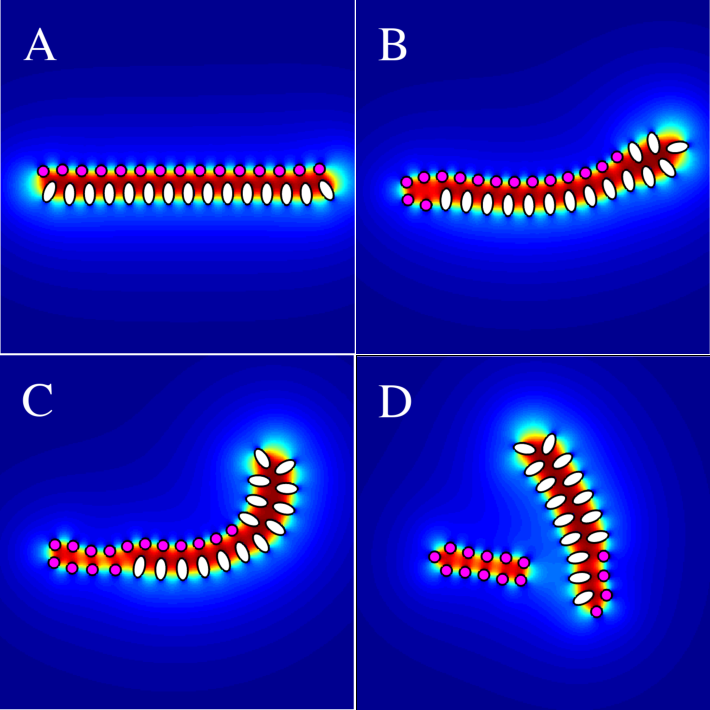
\includegraphics[width=0.4\textwidth]{figures/PW_fig2.pdf}}
%\caption{\label{fig:demixing} An initial assembly of small and 
%large particles spontaneous segregates into two smaller bodies. }
%\end{wrapfigure}
The HAP simulations show vesicle tank-treading. Under the external shear flow, the initially circular 
vesicle rotates in the clockwise direction. As the rate of rotation increases, the vesicle approaches
a steadily tank-treading ellipse. In Figure \ref{fig:tanktreading}B-D, the solid curves are ellipses fit to the particle centers
and midplane respectively. In the non-dimensionalized system, the particles have diameter 2, on the order of $\rho,$ 
and the vesicle diameter is about 14. 
%\todo[inline]{missing units. nm?}
Figure~\ref{fig:tanktreading}E shows the aspect ratio of the major to minor axes reaching an equilibrium value in the 
red and blue curves, yet oscillating in the high-shear rate (yellow) curve.
The tank-treading vesicle elongates and becomes more horizontal 
with an increase in flow rate or 
with a decrease in stiffness (effected by decreasing $\rho = 4$ to $\rho = 2$). 


For large shear flow rates, there is an increase in arc length. Here arc
length refers to the the mid-plane circumference. Thus, some of the
external force is going into stretching the vesicle---the other part is
going into bending and viscous dissipation. From our experiments, we
find that the vesicle ruptures once stretching exceeds about 5 \% (see
Figure \ref{fig:rupture}). Finally, movies of the tank-treading motion
show a slip velocity between the outer and inner leaflets Figure
\ref{fig:tanktreading}G. We have illustrated this by tracking the
distance between two reference particles in the inner and outer leaflet
(Figure \ref{fig:tanktreading}B \& D, green and blue particles). With
moderate shear rates or greater adhesion, the particle pair moves in
tandem (in Figure \ref{fig:tanktreading}H, blue and red curves, their
distance is more or less constant). For a large shear rate, the
particle separates as the two leaflets slide against one another. 



%\begin{wrapfigure}[12]{r}{0.2\textwidth}
%\centerline{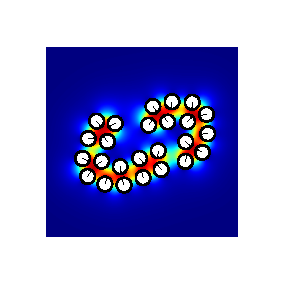
\includegraphics[width=0.2\textwidth]{figures/PW_fig5.pdf}}
%\caption{\label{fig:rupture} Rupture of tank-treading vesicle under strong shear flow.}
%\end{wrapfigure}
%




